\documentclass[class=article, crop=false]{standalone}
\usepackage[subpreambles=true]{standalone}
\usepackage{import}
\usepackage{preamble}
\usepackage{pdfpages}
\usepackage{pgfplots}
\usepackage{pgfplotstable}
\begin{document}
\pgfplotsset{
%        compat=newest,  % <-- does not work; don't know why
        compat=1.13,     % <-- works as expected
    }
  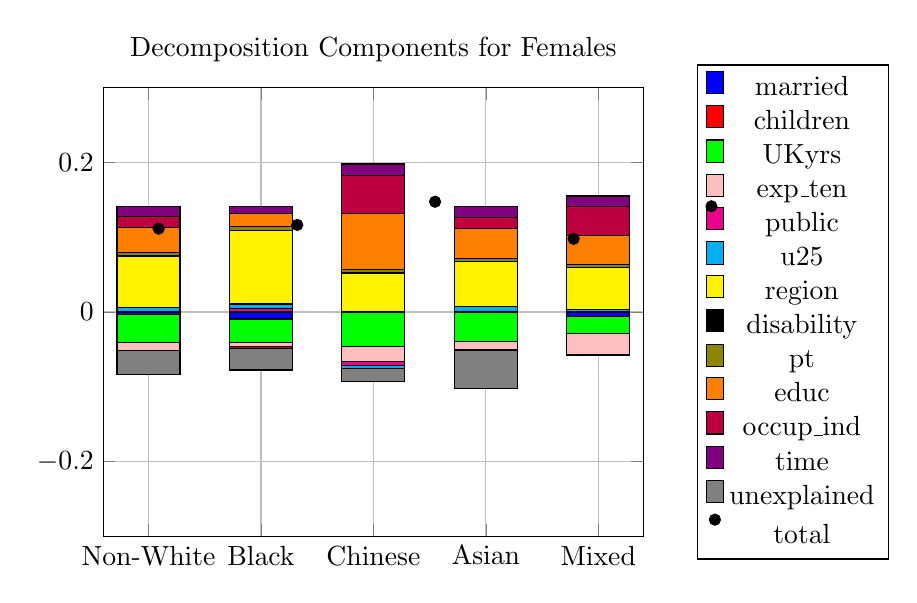
\begin{tikzpicture}
  %\node [align=center, font=\small, rotate=45,text width=2.15cm, inner sep=0.25cm] at (1, 1) {\textsc{year 1}};
  \begin{axis}[
    title={Decomposition Components for Females},
    ybar stacked,
    ymax=0.3,
    ymin=-0.3,
    ymajorgrids = true,
    xmajorgrids = true,
    bar width=8mm,
    %xtick={1,2,3,4,5},
    %xticklabels={White, Black, Chinese, Asian, Mixed}
    symbolic x coords={Non-White, Black, Chinese, Asian, Mixed},
    xtick=data,
    nodes near coords align={anchor=north},%Move values in bar
    every node near coord/.style={},
    legend style={at={(1.1,0.5)},anchor=west}
  ]
%married
\addplot [fill=blue] coordinates {({Non-White},-0.0034119)({Black},-0.0093877)({Chinese},-0.0000912)({Asian},0.0005807)({Mixed},-0.0064773)};
%children
\addplot [fill=red] coordinates {({Non-White},-0.0003497)({Black},-0.0003932)({Chinese},0.0000759)({Asian},-0.0003373)({Mixed},-0.000059)};
%UKyrs
\addplot [fill=green] coordinates {({Non-White},-0.0369829)({Black},-0.0312463)({Chinese},-0.0461203)({Asian},-0.039695)({Mixed},-0.0222872)};
%exp_ten
\addplot [fill=pink] coordinates {({Non-White},-0.010255)({Black},-0.0051381)({Chinese},-0.0196728)({Asian},-0.0098012)({Mixed},-0.0277625)};
%public
\addplot [fill=magenta] coordinates {({Non-White},0.000497)({Black},0.0047931)({Chinese},-0.0059461)({Asian},-0.0011143)({Mixed},-0.001405)};
%u25
\addplot [fill=cyan] coordinates {({Non-White},0.0054961)({Black},0.0059687)({Chinese},-0.0041255)({Asian},0.0066551)({Mixed},0.0037572)};
%region
\addplot [fill=yellow] coordinates {({Non-White},0.0686151)({Black},0.0980698)({Chinese},0.0516301)({Asian},0.0598161)({Mixed},0.0552824)};
%disability
\addplot [fill=black] coordinates {({Non-White},0.0003865)({Black},0.0001804)({Chinese},0.0014378)({Asian},0.0005499)({Mixed},-0.0003162)};
%pt
\addplot [fill=olive] coordinates {({Non-White},0.0042236)({Black},0.0052177)({Chinese},0.0037973)({Asian},0.0035944)({Mixed},0.0049533)};
%educ
\addplot [fill=orange] coordinates {({Non-White},0.034161)({Black},0.0175394)({Chinese},0.0748719)({Asian},0.040029)({Mixed},0.0379698)};
%occup_ind
\addplot [fill=purple] coordinates {({Non-White},0.0144638)({Black},-0.0023758)({Chinese},0.0510769)({Asian},0.015564)({Mixed},0.0387476)};
%time
\addplot [fill=violet] coordinates {({Non-White},0.0128263)({Black},0.009657)({Chinese},0.015264)({Asian},0.0146799)({Mixed},0.0141592)};
%unexplained
\addplot [fill=gray] coordinates {({Non-White},-0.032524)({Black},-0.0290716)({Chinese},-0.0168985)({Asian},-0.0515735)({Mixed},0.0005907)};

\addplot [only marks,mark=*,mark size=2pt,black,
         nodes near coords = \rotatebox{90}{{\pgfmathprintnumber[fixed zerofill,
                                    precision=2]{\pgfplotspointmeta}}},
        nodes near coords align={vertical},
        point meta=y,
        every node near coord/.append style={font=\small, yshift=0.25mm},] coordinates {({Mixed},-1)};
%\begin{comment}
%\end{comment}
%\filldraw[black] (0,0) circle (2pt) node[anchor=west] {Intersection point};
  \legend{married, children, UKyrs, exp\_ten, public, u25, region, disability, pt, educ, occup\_ind, time, unexplained, total}
  \end{axis}
  
  \begin{axis}[
    nodes near coords align={anchor=north},%Move values in bar
    every node near coord/.style={},
    xtick=data,
    ymax=0.3,
    ymin=-0.3,
    xmax=0,
    xmin=5,
]
\pgfplotsset{ticks=none}
\addplot[only marks,mark=*,mark size=3pt,black,
         nodes near coords = \rotatebox{90}{{\pgfmathprintnumber[fixed zerofill,
                                    precision=2]{\pgfplotspointmeta}}},
        nodes near coords align={vertical},
        point meta=y,
        every node near coord/.append style={font=\small, yshift=0.25mm},
        ]  coordinates {
    (1,0.1) (2,-0.1) (3,1)
};
\end{axis}
\filldraw[black] (0.7,3.90573447) circle (2pt) node[anchor=west] {};
\filldraw[black] (2.46,3.95307514) circle (2pt) node[anchor=west] {};
\filldraw[black] (4.21,4.24762574) circle (2pt) node[anchor=west] {};
\filldraw[black] (5.97,3.77653009) circle (2pt) node[anchor=west] {};
\filldraw[black] (7.72,4.1897863) circle (2pt) node[anchor=west] {};
  \end{tikzpicture}
\end{document}